Il tool \textbf{Xilinx\textsuperscript{\textregistered} Vivado\textsuperscript{\textregistered} High-Level Synthesis (HLS)} permette di trasformare le specifiche C in un'implementazione RTL (Register Transfer Level) che può essere sintetizzata e implementata in un FPGA. Pertanto, mediante linguaggi di programmazione ad alto livello come C, C++ e SystemC, è possibile descrivere in maniera più semplice e veloce un'architettura hardware complessa rispetto ad un linguaggio descrittivo dell'hardware come il VHDL o il Verilog. Ovviamente, tale vantaggio si traduce in una minore precisione ed efficienza della descrizione hardware in questione rispetto a quella che si otterrebbe mediante linguaggi HDL. Pertanto, la sintesi ad alto livello dei sistemi digitali risulta essere una congiunzione tra il mondo hardware e quello software. In particolare, tale approccio comporta i seguenti \textbf{vantaggi}:
\begin{itemize}
    \item \textbf{Maggiore produttività per i progettisti hardware}\\
    I progettisti di hardware possono lavorare a un livello di astrazione superiore mentre creano hardware ad alte prestazioni.
    \item \textbf{Migliori prestazioni del sistema per i progettisti di software}\\
    Gli sviluppatori di software possono accelerare le parti computazionalmente intensive dei loro algoritmi su un nuovo target di compilazione, cioè l'FPGA.
\end{itemize}
Inoltre, l'utilizzo di una metodologia di progettazione di sintesi di alto livello consente di:
\begin{itemize}
    \item \textbf{Sviluppare algoritmi tramite linguaggi ad alto livello come C e C++}\\
    Lavorare a un livello astratto dai dettagli di implementazione, che consumano tempo di sviluppo.
    \item \textbf{Verificare il codice mediante compilatori ad alto livello}\\
    Convalidare la correttezza funzionale del progetto in modo più rapido rispetto ai linguaggi di descrizione hardware tradizionali come VHDL e Verilog.
    \item \textbf{Controllare il processo di sintesi C attraverso le direttive di ottimizzazione}\\
    Creare implementazioni hardware specifiche ad alte prestazioni.
    \item \textbf{Creare più implementazioni dal codice sorgente C utilizzando le direttive di ottimizzazione}\\
    Esplorare diversi design per lo stesso progetto permette di trovare implementazioni più efficienti e ottimali.
    \item \textbf{Sfruttare tutti i vantaggi di portabilità e ri-usabilità del codice ad alto livello}\\
    Utilizzare tutte le metodologie ad alto livello basate sull'ingegneria del software e, quindi, risparmiare tempo e costi di progettazione software ulteriori.
\end{itemize}
Per quanto riguarda l'\textbf{HLS Design Flow}, questo si articola nei seguenti passi:
\begin{enumerate}
    \item Compilare, eseguire (simulare) ed eseguire il debug del codice C o C++.
    \item Sintetizzare il codice C in un'implementazione RTL, eventualmente utilizzando direttive di ottimizzazione (pragma).
    \item  Generare e analizzare i report corrispondenti
    \item Packaging dell'implementazione RTL per effettuare l'esportazione dell'IP corrispondente.
\end{enumerate}

\begin{figure}[H]
    \centering
    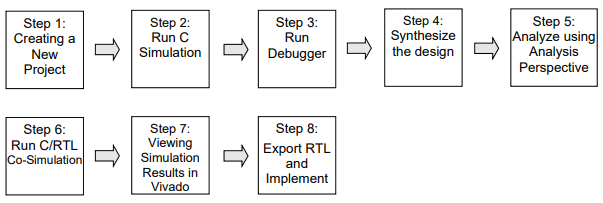
\includegraphics[width=0.6\textwidth]{introduction/designflow.png}
    \caption{HLS Design Flow}
\end{figure}